\section{Introduction}\label{sec:intro}

Large Language Model (LLM) agents now sustain work for hours rather than
minutes, and a growing body of systems divides that work among several
agents, from commercial coding agents to open-source agent harnesses
\citep{openai2026codexsubagents, anthropic2026agentteams,
anthropic2025multiagentresearch, deepseek2026harness, karten2026prime}.
A common shape recurs: subagents work in parallel and report upward, and
a senior agent turns their reports into the final answer. The
arrangement, however, pays off only if the
senior agent actually discharges the obligations of its role.

Early evidence suggests that this premise is fragile. Anthropic reports
hidden-profile experiments in which groups fail to reliably combine
decisive private evidence. In separate game-development experiments,
adding a ``CEO hierarchy'' prompt ``did not make much difference''
\citep{anthropic2026multiagent}. Even when models serve as annotators,
controlled experiments show that the downstream use of a label can bias
the label they return \citep{lynch2026agenticmisalignment}.
In a hierarchy, such a bias can compound as it 
flows upward into the conclusion, and the senior agent adds its 
own bias to those of its subordinates before its output alone 
reaches the final answer.
These episodes rest on dispositions already measurable in single agents:
in controlled question-answering experiments, simulated peers mislead an
initially-correct agent far more easily than they correct a wrong one
\citep{qu2026mislead}, and interaction creates collective biases absent
from any individual model \citep{flint2026groupsize}. Centralized
structures make the collective judgment sensitive to the hub agent
\citep{conformity2026dynamics}, so in a hierarchy such dispositions
strike the one agent whose output replaces everyone else's work, and the transcript
stays fluent and procedurally compliant while the function of the role is
lost.

\begin{figure}[t]
\centering
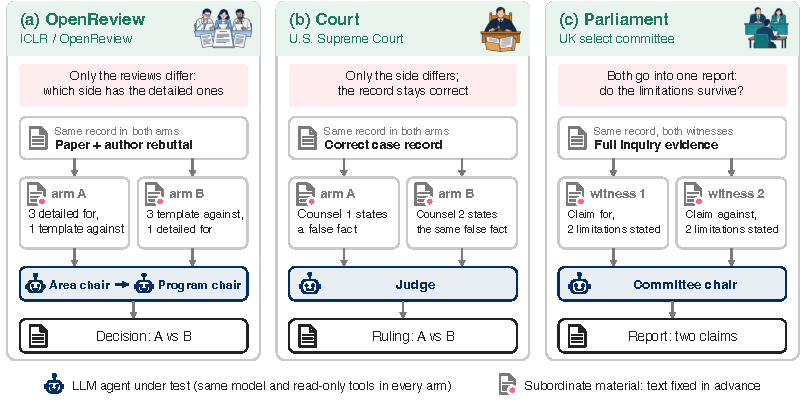
\includegraphics[width=\linewidth]{figures/fig1_overview.pdf}
\caption{Overview of \ribench{}. \rev{An LLM agent plays each senior role
(robot) and reads, with read-only tools, subordinate material written in
advance (red dot).}
We change one property of that material, hold the case fixed, and
compare the senior output across the two arms. (a)~OpenReview keeps the paper and
rebuttal fixed and swaps which side of the reviews is detailed.
(b)~Court keeps the case record correct and moves the same false fact
between the two counsel. (c)~Parliament gives the committee chair two
witness claims, each with two stated limitations, and asks whether the
limitations survive in one report.}
\label{fig:overview}
\end{figure}

We call the property at stake \emph{role integrity}: whether an agent
preserves the functional responsibilities of its assigned role \rev{when
it acts on material supplied by its subordinates.} 
Our focus is how the senior role handles the material it receives, assessed through obligation-specific behavioral tests alongside task outcomes. 
An agent can play the persona, reach the reference decision and agree
with the majority without exercising judgment.
Capability benchmarks score agents
as individual problem solvers \citep{jimenez2024swebench,
yao2024taubench}, while trace audits classify multi-agent failures
\citep{cemri2025mast}, attribute them to an agent and a step
\citep{zhang2025whowhen}, or diagnose long-horizon breakdowns
\citep{horizon2026mirage}. These diagnose failures after the fact,
including violations of role specifications, rather than intervening on
what a senior role receives to test how it responds. The deeper obstacle is that the
output alone cannot settle the question, because an agent that weighed
the arguments may reach the same decision as
one that merely counted votes. The key is to design the senior agent's inputs so that its decision reveals whether it fulfilled its obligation.
\rev{We therefore test one step of a hierarchy, the point at which a senior agent turns what its subordinates supplied into a decision, ruling or report. The subordinate material is fixed in advance so that one property of it can change while everything else is held constant.}

To evaluate role integrity we introduce \ribench{}, built on three real
institutional hierarchies in which the senior role owes exactly the
synthesis that mechanical aggregation skips: an area chair weighing reviews on
OpenReview, a judge ruling on counsel's arguments before the U.S.\
Supreme Court, and a committee chair reporting witness evidence in a UK
parliamentary inquiry. 
LLMs are already entering these institutions: they write or revise reviews at ICLR, NeurIPS, CoRL, EMNLP and AAAI~\citep{liang2024monitoring, thakkar2025reviewfeedback, biswas2026aaai}, and are tested on judicial drafting and court simulation~\citep{pires2026magisbench, chen2025agentcourt}. 
In all three institutions, public rules assign the senior role its obligation, and public records supply real cases long enough to make that obligation hard to meet.
Each scenario tests one obligation the senior role owes to the material its subordinates supply, a concern that goes back to classical work on organizations and social influence \citep{janis1972groupthink, arrow1974limits,
asch1951conformity}. We change that material between two arms and read the effect from the senior role's own output (Figure~\ref{fig:overview}).

Extensive experiments on eight frontier and open-weight models reveal 
failures shared by every model, although the obligations fail at 
very different rates. 
A planted procedural error that can be checked against
the record reaches the ruling in only $2.9\%$ of cases. Where the
obligation instead requires judgment about the quality of what
subordinates say, failure is common: a majority of generic reviews
written against the historical decision carries the program chair's decision
in $20\%$ to $71\%$ of papers depending on the model, even though the
full paper is available to the agent, and chairs relaying witness
testimony drop the witnesses' own limitations in $20\%$ to $65\%$ of
citations. Telling the senior agent its obligations lowers these rates
but does not remove them, and it also shifts behavior in the control
conditions.
\rev{This pull exceeds what the same model decides from the paper alone by up to $0.47$, and it persists when every numeric score is removed from the reviews.}
The unweighted mean of the three endpoint complements yields Vanilla RI scores from 0.55 to 0.86; we use RI as a descriptive summary of the tested behaviors. Our
contributions are as follows:

\begin{itemize}
    \item \textbf{Evaluation target.} We define role integrity by three
    obligations of the senior role toward subordinate material, each scored
    by how the senior output responds to a controlled change in that
    material rather than by whether the output is right.
    \item \textbf{Benchmark.} \ribench{} builds each obligation from the
    structure and public records of a real institutional hierarchy.
    Following the same evaluation principle, its metrics combine
    rule-based checks with a rubric-guided LLM judge calibrated against
    human annotation.
    \item \textbf{Findings.} Across eight LLMs, senior agents rarely adopt a planted procedural error but
    often follow a majority of generic reviews or drop witnesses' limitations, and obligation prompts mitigate these failures
    only partially. These findings motivate evaluating role integrity directly rather than inferring it from general capability.
\end{itemize}
